\documentclass[a4paper,12pt]{report}
\usepackage[utf8]{inputenc}
\usepackage{graphicx}
\usepackage{amsmath}
\usepackage{multirow}
\usepackage{tikz}
\setcounter{secnumdepth}{3}
\usepackage{pdfpages}
\usepackage{tabto}
\usepackage[nottoc,notlof,notlot]{tocbibind} 
\renewcommand\bibname{References}
\usepackage{cite}
\usepackage{color}
\usepackage{algorithm,algpseudocode}
%\usepackage{algorithm2e}
%\usepackage{algpseudocode}
%\SetKwInOut{Parameter}{parameter}
\renewcommand{\baselinestretch}{1.3}
%\usepackage[document]{ragged2e}
\usepackage[pages=some]{background}
%\usepackage{romannum}
\usepackage{kantlipsum}
\usetikzlibrary{shadows,fadings}
\usepackage{xcolor}

%opening
\backgroundsetup{%
  scale=1,       %% change accordingly
  angle=0,       %% change accordingly
  opacity=.08,    %% change accordingly
  color =black,  %% change accordingly
  contents={\begin{tikzpicture}[remember picture,overlay]
        \node at ([yshift=11pt,xshift=5pt]current page.center) {\includegraphics[width=15cm]{images/NIT_Goa_Logo.png}};    %% yshift and xshift for example only
    \end{tikzpicture}}
}


\begin{document}

\begin{titlepage}
\begin{center}
       
       \Large {\textbf{Face Recognition with Masks using Bio-Inspired Algorithm}
}
        
     \vspace{0.2cm}
     {\footnotesize Project Report Submitted in Partial Fulfillment of the Requirements for the Degree of}\\
     \vspace{0.2cm}
   
    
     \textbf{\large Bachelor of Technology}\\
        {\textit{in}}\\
           \textbf{\Large Computer Science and Engineering}
           
           \vspace{0.5cm}
           
           \textit{Submitted by}\\
        \textbf{\large Anit Mahato:(roll no. 17CSE1004)}\\
         \textbf{\large Gautam Mishra:(roll no. 17CSE1011)}\\
          \textbf{\large Sangram Patil:(roll no. 17CSE1030)}
        \vspace{1cm}
                
        \centering \large {\textit{Under the Supervision of}}\\
        \textbf{\large Dr. Venkatanareshbabu Kuppili}\\
         \centering{Assistant Professor}
         \vspace{0.5cm}
     
      \includegraphics[width=0.26\textwidth]{images/NIT_Goa_Logo.png}\\
        \vspace{0.2cm}
        
       \textbf{Department of Computer Science and Engineering}\\
       \vspace{0.1cm}
        \textbf{National Institute of Technology Goa}\\
    %   \vspace{0.3cm} 
 
        \centering{Nov,2020}
    \end{center} 
\end{titlepage}


\thispagestyle{empty}
\BgThispage
\begin{table}[]
\centering
%\caption{My caption}
\label{my-label}
\begin{tabular}{lc}

\parbox[c]{1em}{
      \includegraphics[scale=0.27]{images/NIT_Goa_Logo.png}} & \begin{tabular}[c]{@{}c@{}} 
      \hspace{20mm}   
      {\textbf{{Department of Computer Science and Engineering}}}\\
  \hspace{52mm}    
\small{\textbf{{National Institute of Technology Goa}}}\\
\hspace{67mm}
\small{\textbf{{Farmagudi, Goa, India-403401}}}
\end{tabular}
\end{tabular}
\end{table}
\vspace{-15mm}
 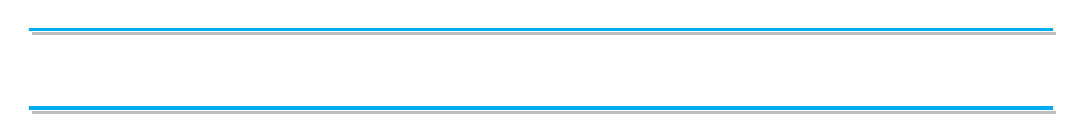
\begin{tikzpicture} 
 \tikzset{
    shadowed/.style={preaction={transform canvas={shift={(1pt,-1.5pt)}},draw=lightgray,very thick}},
  }
   \draw[cyan, very thick, rotate=0, shadowed] (0,0) -- (13,0);
   \draw[cyan, very thick, rotate=0, shadowed] (0,-1) -- (13,-1);
\end{tikzpicture}

%\hline
\vspace{-13mm}
\begin{center}
\begin{normalsize}
\textbf{CERTIFICATE}\end{normalsize}
\end{center}
\vspace{0.3cm}
\noindent This is to certify that the work contained in this report entitled \textbf{“Face Recognition with Masks using Bio-Inspired Algorithm”} is submitted by the group members Mr. Anit Mahato (Roll. No: 17CSE1004), Mr. Gautam Mishra (Roll. No: 17CSE1011) and Mr. Sangram Patil (Roll. No: 17CSE1030) to the Department of Computer Science and Engineering, National Institute of Technology Goa, for the partial fulfillment of the requirements for the degree of \textbf{Bachelor of Technology} in \textbf{Computer Science and Engineering}.\\
\\
They have carried out their work under my supervision. This work has not been submitted else-where for the award of any other degree or diploma.\\
\\
The project work in our opinion, has reached the standard fulfilling of the requirements for the degree of Bachelor of Technology in Computer Science and Engineering in accordance with the regulations of the Institute.
\vspace{2cm}
\begin{flushleft}
\textbf{(Supervisor(s))}\\ Department of CSE\\ NIT Goa
\end{flushleft}
\begin{flushright}
\textbf{(HoD)}\\ Department of CSE\\ NIT Goa
\end{flushright}
\pagebreak



% \section*{\centering Acknowledgment}
% Some text here....
% \pagebreak
%  \pagenumbering{roman}


% ---------------------------------------Abstract-----------------------------------

\section*{\centering Abstract}
The use of these face masks has raised a serious question on the effectiveness of the facial recognition system that is used in tracking attendance and mobile phones to unlock them or in surveillance. Here, we are devising a solution which can effectively identify a person with or without a mask. We will be using bio-inspired algorithms to get the best set of features out of numerous extracted features with the deep neural network. 


% -------------------------------------Table of Content-----------------------------

\tableofcontents
\listoffigures
% \listoftables
\pagebreak
\pagenumbering{arabic}

% -------------------------------------Introduction---------------------------------

\chapter{Introduction}
As we know the Corona Virus or Covid-19 has devastated the world. It is a highly communicable virus. The most common way of its spreading is through the air we breathe. To prevent these people nowadays wear masks when they are in public places. Wearing such masks has made the job of face recognition systems harder than before. Face recognition systems are used for identity authentication, security access control, and intelligent human-computer interaction. Under CCTV surveillance if a perpetrator wears a mask, security face recognition techniques might not work. Face recognition bio-metic are also not usable. In such cases, we need an effective way to identify the face of a person without them removing the mask. So we need an improvised Face Recognition technique which can recognise faces over face mask.

\section{Problem Statement}
The face recognition systems are not prepared for occlusion. The algorithms are not able to extract enough features form a masked-face. We are devising a face recognition system which works even with face masks. Here, we will be using bio-inspired algorithms to recognise faces with a mask. 

% Adding and Image
% you can add an image as below
% \begin{figure}[h]
% \center
%  \includegraphics[width=0.5\textwidth]{images/NIT_Goa_Logo.png}
%  \caption{image caption}
% \end{figure}
% \subsection{Your subsection here}
% Some subsection part here
% \subsubsection{Your subsubsection here}
% Write here sub sub section 

\pagebreak

% -------------------------------------Related Work---------------------------------


\chapter{Related Work}
There are some existing research work on face recognition with occlusion \cite{conference6}.\\
The question is still the same, what featues should be extracted that are useful. Feature extraction algorithms mainly fall into two categories: geometrical features extraction and statistical (algebraic) features extraction \cite{conference5}. The geometrical features extraction represents the face in terms of structural measurements like distance between eye and nose\cite{conference3}. Whereas statistical features extraction represents faces like eigenvectors in case of Principal component analysis (PCA) or Independent component analysis (ICA), or mean and standard deviation in case of descriptive statistics\cite{conference1}.\\
In the feature selection stage we search for the most optimal subset of features out of all the extracted features. One possible solution would be to do a brute force and search among all the possible subsets which is computationally expensive and impractical. Among the feature selection algorithms the Partical Swarm optimization(PSO) and Ant Colony Optimization have achieved good results\cite{conference7}. Here, we will be using face recognition with mask using PSO based feature selection algorithm. 


% -------------------------------------Proposed Method-----------------------------

\chapter{Proposed method}
Due to the curse of dimensionality, we can not use algorithms like SVM or deep learning. We can solve this problem by dimensionality reduction techniques.

Preparation the Dataset: The face recognition algorithms require a large amount of training data but there is no standard dataset available in the public domain for face recognition with mask. We have used the standard face recognition dataset and mixed some images with the augmented face mask. On a face we first identify all the facial key points, mask the region below eye and augment the mask on this region. Using this approach we can use existing face recognition datasets and augment the face masks for some percentage of images say 70\% and rest of the images will be without face masks for every identifiable person.

\begin{figure}[h!]
\center
 \includegraphics[width=0.7\textwidth]{images/Dataset preparation.png}
 \caption{Dataset preparation}
\end{figure}

After obtaining the dataset, we extract the relevant features out of descriptive statistics, geometrical features, or eigenfaces as discussed in the previous section. From these extracted features, we select the most useful features using a bio-inspired optimization algorithm, particularly Particle swarm Optimisation (PSO) and Deep neural networks. This reduces the noise and selects only a subset of the original features which are most useful out of the whole search space. After obtaining the feature matrix we save all the training examples embedding to our face gallery which will be later used for prediction. \\

During the testing phase, we use the recognition matrix to calculate the embedding vector. We compare this embedding with our face gallery embedding using some metric. We take the 'argmax' of these results which gives us the identified face.

\begin{figure}[h]
\center
 \includegraphics[width=1\textwidth]{images/mp_flowchart.png}
 \caption{Process flow}
\end{figure}

% -------------------------------------RESULT--------------------------------------

% \chapter{Results}
% Some results here.....

% \begin{table}[ht]
% \centering
% \caption{Table1}
% \label{my-label}
% \begin{tabular}{|l|l|l|}
% \hline
% Parameter1 & Parameter2 & Parameter3 \\ \hline
% write value here & value2 & value3 \\ \hline
% value1 & value2 & value3 \\ \hline
% \end{tabular}
% \end{table}

% -------------------------------------The Optimization Methods-----------------------------------
\chapter{The Optimization Methods}
We intend to reduce the features extracted further for more improved efficiency. In this project we would be using Bio-Inspired Algorithms for Optimization. The two most renowned techniques for Bio-Inspired Algorithms are the Particle Swarm Optimization(PSO) and the Genetic Algorithm(GA). In the following, exhaustive description of both algorithms are given along with their pseudo codes.

\section{Genetic Algorithm}
Genetic Algorithm is an evolutionary algorithm inspired by Darwinian evolution biology. It is composed of a population of individuals randomly generated in the search space, represented by a specific encoding and stands for the feature vector (after extraction) in context to this project. At each iteration, each individual is evaluated, and/or selected to produce a new population to be used for the next iteration. The evaluation of every individual is performed by the feature index to be optimized. The reproduction of new individuals is done as follows. A tournament selection of n participants (n=3) and a k-point crossover (k=2) with a probability equal to greater than 0.5 ideally (significantly large probability because crossovers are necessary for the next generation) applied to the entire population.\par
\noindent Once the selection and the crossover stages are achieved, a different (new) population of individuals is generated either immediately copied or created by crossover. Finally, a mutation operator is employed to each individual using a probability equal to less than 0.1 ideally (extremely small probability because the chances of mutation are very rare) by choosing arbitrarily one gene to be substituted by a random real value.\par
\begin{flushleft}
\noindent \textbf{Algorithm:}\\
\begin{enumerate}
\item \textbf{Begin} Genetic Algorithm
\item \textbf{While Not Stop Do}
\item Initialize the population at random,
\item \textbf{Begin}
\item  Select individual, by a tournament process by mating;
\item  Apply the crossover operator to create the new individual;
\item  Apply mutation operator on the new individual created at 2;
\item  Compute the fitness of the individual;
\item  Insert this individual into the population, and remove the individual with the lowest fitness;
\item  Check if Stopping Criteria are satisfied;
\item \textbf{End}
\item Output best individual;
\item \textbf{End} GA Algorithm;
\end{enumerate}
\end{flushleft}
\pagebreak

\section{Particle Swarm Optimization}
Particle Swarm Optimization is a population based stochastic optimization method inspired by social behaviour of bird flocking or fish schooling. In PSO, a population called “swarm” is initialized by random particles covering the search space. The particle represents the feature vector in context to this project. Every particle is assessed by means of the feature index to be optimized. The position of each particle is updated at each iteration according to its best position achieved so far (called pbest), the best position of the best particle of the swarm (called global best and denoted by gbest) and the velocity which is randomly initialized. Moreover, the particle position may be concerned by its neighbours, especially the best neighbour particle (called the local best and denoted by lbest). In this case, the particles do not investigate the entire search space but move in near vicinity to the local best. As soon as the positions of all the particles are updated, this configuration is updated by the formation of novel groups. The number of iterations and the number of individuals/particles are chosen so that the obtained optimum is difficult to be enhanced (using numerous tests).

\begin{flushleft}
\noindent \textbf{Algorithm:}\\
\begin{enumerate}
    \item Swarm size is \textbf{N}
    \item Max number of iterations is \textbf{max\_iterations}
    \item \textbf{getBestNeighbour}: a function to get a particle’s best neighbour (lbest) among the number of neighbours =3
    \item \textbf{rand( )}: is a random number uniformly distributed in [0,1];
    \item \textbf{C1}=0.7
\end{enumerate}
\pagebreak
\begin{flushleft}
\quad \textbf{while} (iteration number $\leq$ \textbf{max\_iterations})\\
\quad \{\\
\quad \quad \textbf{while} (Number of particles $\leq$ \textbf{N})\\
\quad \quad \{\\
\quad \quad \quad Update position: \textbf{position} = position + Velocity\\
\quad \quad \quad Calculate fitness\\
\quad \quad \quad If (fitness $>$ fitness(pbest))\\
\quad \quad \quad \{\\
\quad \quad \quad \quad \textbf{fitness(pbest)} = fitness\\
\quad \quad \quad \quad Update the best position: \textbf{pbest} = position (newly\_updated)\\
\quad \quad \quad \}\\
\quad \quad \quad Update the best neighbor: \textbf{lbest} = getBestNeighbour()\\
\quad \quad \quad Update Velocity: \textbf{Velocity} = C1.Velocity + rand( ).(pbest-position)\\ 
\quad \quad \quad + rand( ).(lbest-position)\\
\quad \quad \}\\
\quad \}\\
\end{flushleft}

\quad 

\end{flushleft}



% -------------------------------------Conclusion-----------------------------------

\chapter{Conclusion}
This project will help the society to improve their security systems in current times. People no longer have to take their masks off for face bio-metrics machines. We have generated the dataset effectively by augmenting digital face masks on the face recognition dataset. Thus, we were able to produce a good number of examples for training. The BPSO is an efficient Optimisation technique which selects a subset of most relevant and useful features from the entire set of features. We will be using a Deep Neural Network with BPSO that produces an encoding which we save to our database of face gallery for prediction. During the testing phase, we again obtain the extracted features, calculate recognition feature matrix and find the closest embedding from the face gallery. 


% -------------------------------------References-----------------------------------


\begin{thebibliography}{15}

\bibitem{conference1} Rojana Kam-art, Raicharoen, T., \&; Khera, V. (2009). "Face recognition using feature extraction based on descriptive statistics of a face image". \textit{2009 International Conference on Machine Learning and Cybernetics}.

\bibitem{conference2}Wang, S., Wen, G., \&; Cai, H. (2017). "Feature extraction and face recognition algorithm." \textit{2017 13th  International Conference on Natural Computation, Fuzzy Systems and Knowledge Discovery (ICNC-FSKD)}.

\bibitem{conference3}Benedict, S. R., \&; Kumar, J. S. (2016). "Geometric shaped facial feature extraction for face recognition". \textit{2016 IEEE International Conference on Advances in Computer Applications (ICACA)}.

\bibitem{conference4}Santhosh Shetty , Paritosh Kelkar , K Manikantan , S Ramachandran. \textit{International Conference on Computational Intelligence: Modeling, Techniques and Applications (CIMTA) 2013} "Shift Invariance based Feature Extraction and Weighted BPSO based Feature Selection for Enhanced Face Recognition".

\bibitem{conference5}Ramadan, R. M., \& Abdel-Kader, R. F. (2009). Particle swarm optimization for human face recognition. 2009 IEEE International Symposium on Signal Processing and Information Technology (ISSPIT).

\bibitem{conference6}H. Jia and A. M. Martinez, "Face recognition with occlusions in the training and testing sets," 2008 8th IEEE International Conference on Automatic Face \& Gesture Recognition, Amsterdam, 2008, pp. 1-6, doi: 10.1109/AFGR.2008.4813410.

\bibitem{conference7}Rashidy Kanan, Hamidreza \& Faez, Karim \& Hosseinzadeh Aghdam, Mehdi. (2007). Face Recognition System Using Ant Colony Optimization-Based Selected Features. Proceedings of the 2007 IEEE Symposium on Computational Intelligence in Security and Defense Applications, CISDA 2007. 57 - 62. 10.1109/CISDA.2007.368135. 

\bibitem{conference8}"Face Identification based Bio-Inspired Algorithms"
Sanaa Ghouzali and Souad Larabi 
Department of Information Technology, King Saud University, Saudi Arabia
Computer Science Department, Prince Sultan University, Saudi Arabia doi:10.34028/iajit/17/1/14
\end{thebibliography}
\pagebreak 

\end{document} 